\chapter{A New Approach}

In this chapter, we will present a noval approach for rendering a scene with dynamic light source efficiently. This method is based d on the standard GPU-based photon mapping rendering system, using an augmented kd-tree data structure and localized updating algorithm for rendering.  

In the first 2 sections of this chapter, We will have an overview on our approach and comprehensive description of the data structure that we use and related algorithms. Then we will look at some of the GPU implementation details. 

\section{Overview} 

As described in chapter 2, we build a gloabl kd-tree as the photon map for irradiance estimation. However, the global photon map is rebuilt from scratch every frame, this process is time consumings due to the complexity of kd-tree building algorigthm on GPUs and can be avoided. 

Instead of building a global kd-tree for photons, we re-use the same kd-tree for the geometry objects(triangles) which is static and associate the geometry and the photons data for efficient KNN search and update for dynamic scene. 

For each frame, the photons are shot from the light source and stored in an array, then we build the kd-tree for the geometry objects if it is required, for the scenes that don't include animated objects we will skip this process. Given the photons data in the scene and the built kd-tree for geometry, we build our data structure, compress the memory bind it to the texture memory for a better memory accessing performance. In rendering phase, instead of using photon map for radiance estimation, we use the kd-tree and our photon queue perform KNN search. Further details of the data structure will be presented in the following section. 

The update process of photons queue is straightforward. It depends on the photon data from the previouse frames. Here we keep track of all the photons data of a range of frames with a pair of indices, the indices can be updated and maintained efficiently. Furthur  details will be presented in following section.  

\section{Data Structure And Algorithm} 

\subsection{Data Structure}

\begin{figure}[htp] 
    \centering 
    \fbox{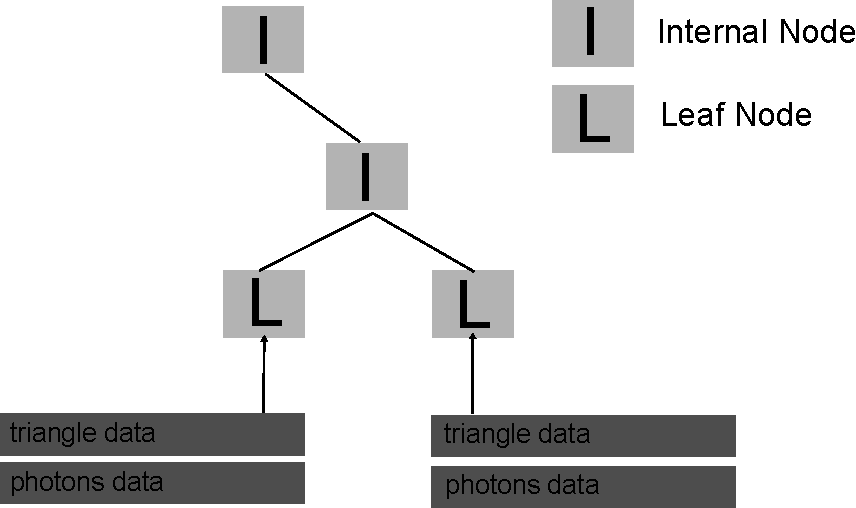
\includegraphics{kd_leaf_photons.pdf}}
    \renewcommand{\thefigure}{\thechapter.\arabic{figure}}
    \caption[]{Radiant flux from a point light source is passing through the spheres around the light.}
    \label{fig:kd_leaf_photons} 
\end{figure}  

As shown in figure \ref{fig:kd_leaf_photons}, in addition to the triangle data, the photons data in the scene is also logically associated with the leaf nodes of the kd-tree. As the kd-tree for the scene actually encodes the spatial relationship among the geometry, and the photons will be stored when they hit the objects with diffuse objects, we attach the photons fall into the spatial region occupied by the bouding box of a kd-tree leaf node. 

\begin{figure}[htp] 
    \centering 
    \fbox{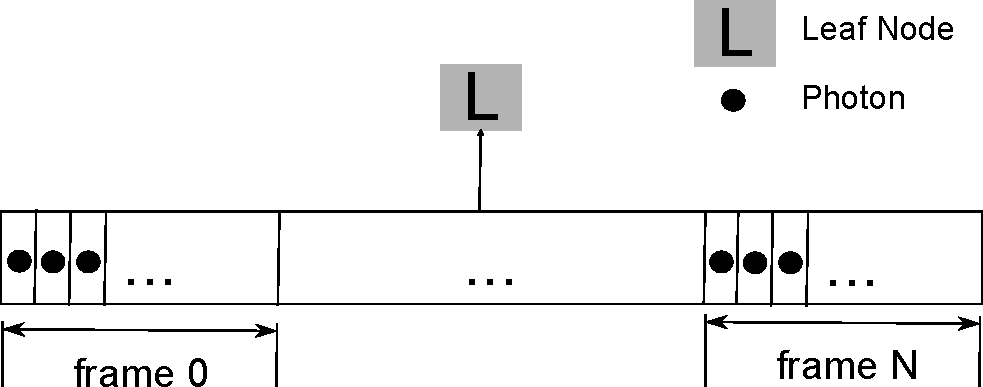
\includegraphics[width=\linewidth]{kd_leaf_photons_2.pdf}}
    \renewcommand{\thefigure}{\thechapter.\arabic{figure}}
    \caption[]{Radiant flux from a point light source is passing through the spheres around the light.}
    \label{fig:kd_leaf_photons_2} 
\end{figure}  

In figure \ref{fig:kd_leaf_photons_2} we have a more detailed view on how the photons data organized. The photons shot to the scene in one frame of rendering are stored followed by the photons of next frame. When implementing this organization on GPU, all actual photons data (positions, incident directions and power) is stored in a seperate array, the indices of the photons associated with kd-tree leaf nodes are stored instead of the actual photon data. 

\subsection{Construction} 

Building the logical connection between photons and leaf nodes is simpler than build a global kd-tree for the photon map. Firstly, we found out the the leaf nodes from the built kd-tree in parallel. This can be done checking a flag set when building the kd-tree. Given the indices of leaf nodes, we can retrieve the bounding box from the small node list generated in kd-tree construction phase(see \ref{subsec:kdtree_construction}). Then we check which leaf node certain group of photons should fall into in parallel by performaing fast point-box intersection testing. For each leaf node, the number of photons can be calculated with a parallel reduction operation. Further details on physical memory arrangement and implementation of the data structure  will be presented in section \ref{sec:impl_detials}. 

\subsection{Update} 

When a frame of image is rendered, new photons will be shot into the scene and be stored in the same global array with previous frames and for each leaf node, we need to keep track of the range of the photons that are active for rendering the next frame. For each leaf node, we maintain two pointers(indices), start and end index, indicating the range of the photons used for rendering. We move the end pointer forward as there are new photons comming, move the start pointer forward when there are some old photons we need to discard. We use a pre-defined threshold fram count to determine how manay frames of photons data we want to make active, we keep accumulating the photons every frame until we reach that threshold value. When the threshold frame count 
is reached, we move forward the start pointer to avoid there are too many photons than there should be. Since the number of photons per frame is known, the stride of moving start pointer can be calculated. However, in GPU implementation, the step in bytes used to increment the pointer is usually larger than the exact size of photons data we want to discard, since the memory will be padded when it is allocated for better memory accessing performance. Further details will be presented in section \ref{sec:impl_detials}. 

\subsection{Rendering} 

Rendering with our data structure does not differ from the standard photon mapping rendering algorithm. In rendering phase, we cast the rays from the camera into the scene in parallel and perform KNN search using the kd-tree already built for the geometry, when we reach the leaf nodes we use our data structure to find the photons data for particular leaf node and gather the photons for radiance estimation. 

\section{Implementation Details} 
\label{sec:impl_detials} 

\subsection{Data Organization}

\paragraph{KD-Tree Data} 

The kd-tree data should be carefully organized when implemented with CUDA to improve traversal performance. In \ref{subsec:kdtree_construction}, we have already described the kd-tree building algorithm introduced in \cite{Zhou2008}, but some of the details that are critical to the program's overall performance still need to be discussed here. 

The final node list generated when the kd-tree is built is not sufficient for fast traversal algorithm, it contains too much useless information and will hit the performance since it is not friendly to cache prefetch. Therefore we compress and re-organize the traversal related data of the kd-tree nodes to reduce the memory access. The entire kd-tree is stored in a structure of several contiguous arrays. The structure is defined as following:  

\lstinputlisting{kdtree_data_def.cpp} 

of unsigned integer and is organized in pre-order, as shown in the following figure: 

\begin{figure}[htp] 
    \centering 
    \fbox{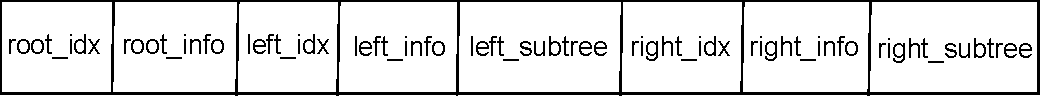
\includegraphics[width=\linewidth]{kdtree_data_memory_layout.pdf}}
    \renewcommand{\thefigure}{\thechapter.\arabic{figure}}
    \caption[]{Compacted kd-tree data memory layout.}
    \label{fig:kdtree_data_memory_layout} 
\end{figure}  

The whole left subtree is stored before right child and its subtree due to the pre-order traversal, this memory layout improves the cache performance. 


\paragraph{Photons Data} 


\subsection{GPU memory management}


\paragraph{GPU Texture Memory VS Global Memory} 


\paragraph{Shared Memory} 






